% --- Ejercicio 1 -------- %
\begin{ejercicio}
    Aplique el mapeo lineal $w = (\sqrt{3}+j)z-j$ a la figura \ref{fig:map1}.
    \label{ej:1}
\end{ejercicio}

\begin{figure}[!h]
    \centering
    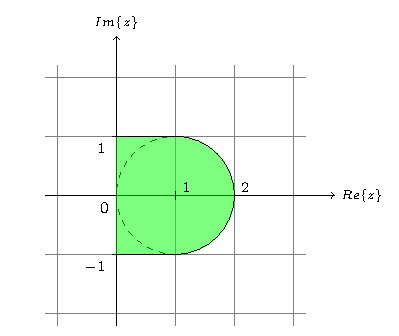
\includegraphics[width=.5\linewidth]{figs/map1.pdf}
    \caption{Plano z para ejercicios \ref{ej:1} y \ref{ej:2}.}
    \label{fig:map1}
\end{figure}

% --- Ejercicio 2 -------- %
\begin{ejercicio}
    Aplique el mapeo de inversión a la figura \ref{fig:map1}.
    \label{ej:2}
\end{ejercicio}

% --- Ejercicio 3 -------- %
\begin{ejercicio}
    Aplique el mapeo bilineal $w = -2 + \frac{j4}{2z+j}$ a la figura \ref{fig:map2}.
    \label{ej:3}
\end{ejercicio}

\begin{figure}[!h]
    \centering
    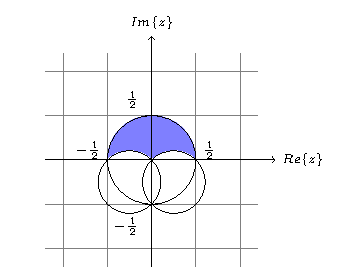
\includegraphics[width=.6\linewidth]{figs/map2.pdf}
    \caption{Plano z para ejercicio \ref{ej:3}.}
    \label{fig:map2}
\end{figure}

% --- Ejercicio 4 -------- %
\begin{ejercicio}
    Encuentre a qué corresponde en el plano $w$ la región del plano $z=x+jy$ dada por $y \geq 0$ bajo el mapeo:
    $$ w = f(z) = e^{j\theta} \frac{z-z_0}{z-z_0^*} $$
    Para ello, encuentre los valores particulares de $\theta$ y $z_0$ si se cumple que $f(j)=0$ y $f(\infty) = -1$.
\end{ejercicio}

% --- Ejercicio 5 -------- %
\begin{ejercicio}
    Encuentre un mapeo bilineal $w=f(z)$ que transforme a la curva A del palno $z$ mostrada a la izquierda de la figura \ref{fig:map3-4}, en la curva B del plano $w$ mostrada a la derecha, si se sabe que la sección de la curva A ubicada sobre $|z-1| = 1$ es transformada en el segmento de recta que une $-1$ y $1$ en el plano $w$.
    \label{ej:5}
\end{ejercicio}

\begin{figure}[!h]
    \centering
    \subfigure[Plano $z$.]{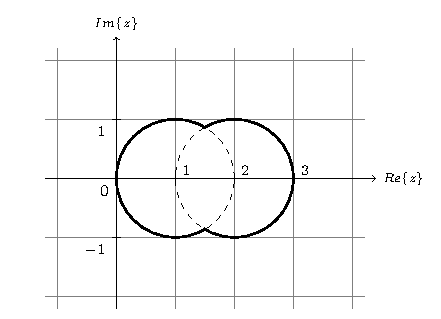
\includegraphics[width=0.465\linewidth]{figs/map3.pdf}}
    \subfigure[Plano $w$.]{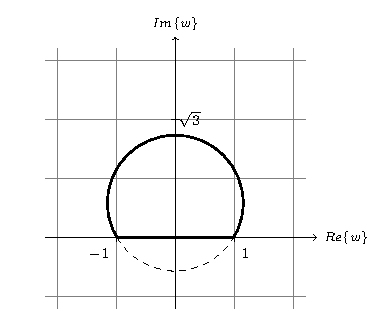
\includegraphics[width=0.4\linewidth]{figs/map4.pdf}}
    \caption{Planos $z$ y $w$ para ejercicio \ref{ej:5}.}
    \label{fig:map3-4}
\end{figure}

% --- Ejercicio 6 -------- %
\begin{ejercicio}
    Describa en el plano $w$ la imagen de la recta $x=\beta$ ($\beta$ constante) del plano z bajo el mapeo $w=z^2$.
\end{ejercicio}
